%!TEX root = ../Master_template.tex
\chapter{Methodology}

This chapter introduces our proposed augmentation methods by outlining the motivation behind them and the inspiration drawn from other domains that led to their design. It presents the method for time series forecasting, along with two different variants tailored for time series classification. The chapter concludes by providing a rationale for the methodology and its underlying design objectives.

\section{Motivation}


Patch-based augmentations have become quite common in Computer Vision (CV), especially for their effectiveness in data augmentation and regularization. These techniques split the input images into multiple patches and implement transformations in these patches to improve model generalization and robustness. Two recent examples are PatchMix~\cite{hong2024patchmix} and PatchShuffle~\cite{kang2017patchshuffleregularization}, which contributed to the design of our proposed augmentation strategies for time series data. According to the authors, these methods improve the generalizability of the models by encouraging them to learn more robust and spatially invariant features. Additionally, they act as regularizers, helping to reduce overfitting in scenarios where training data is limited~\cite{kang2017patchshuffleregularization, hong2024patchmix}.



Figure~\ref{fig:patchmix} illustrates the PatchMix augmentation method. As an example, the input image is divided into four non-overlapping patches. These patches are then shuffled and recombined using a MixUp-like strategy, where the combination weights are drawn from a Beta distribution. An important feature of PatchMix is that the mixing process introduces patches that may bypass the mixing step and go directly to the final composition, making the resulting image more diverse. The authors also proposed a variant called PatchMix-R, which is inspired by PatchShuffle. The only difference lies in the mixing step: PatchMix-R performs local mixing of nearby pixels within patches rather than entire patches~\cite{hong2024patchmix}.



\begin{figure}[h!]
    \centering
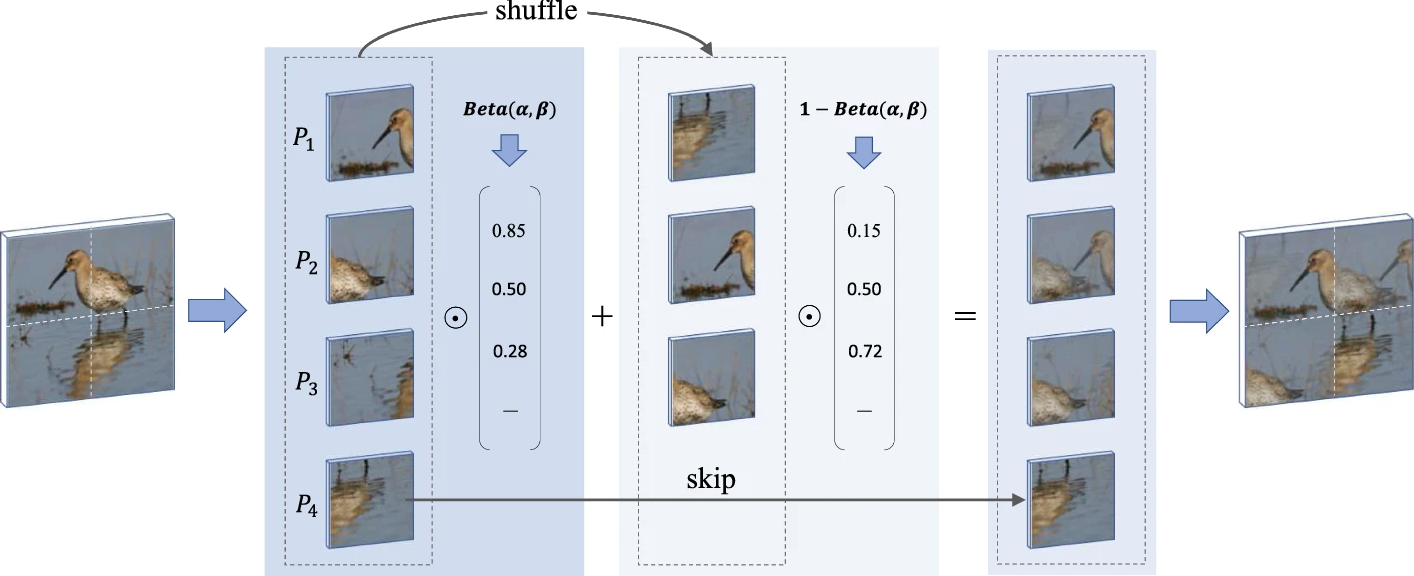
\includegraphics[page=1, width=0.9\textwidth]{./images/patchmix.png}
\caption{PatchMix augmentation. The input image is split into non-overlapping patches, which are shuffled and combined using MixUp-style weights from a Beta distribution. Some patches may bypass mixing for added diversity~\cite{hong2024patchmix}.}
    \label{fig:patchmix}
\end{figure}



Figure~\ref{fig:patchshuffle} presents a simplified version of the PatchShuffle method. In this example, a $4 \times 4$ image matrix is divided into four non-overlapping $2 \times 2$ patches. The pixels within each patch are independently shuffled: attributes in each patch are permutated separately, and a shuffled patch may also have its original structure. This local pixel-level shuffling introduces variation while preserving the global structure of the image~\cite{kang2017patchshuffleregularization}.



\begin{figure}[h!]
    \centering
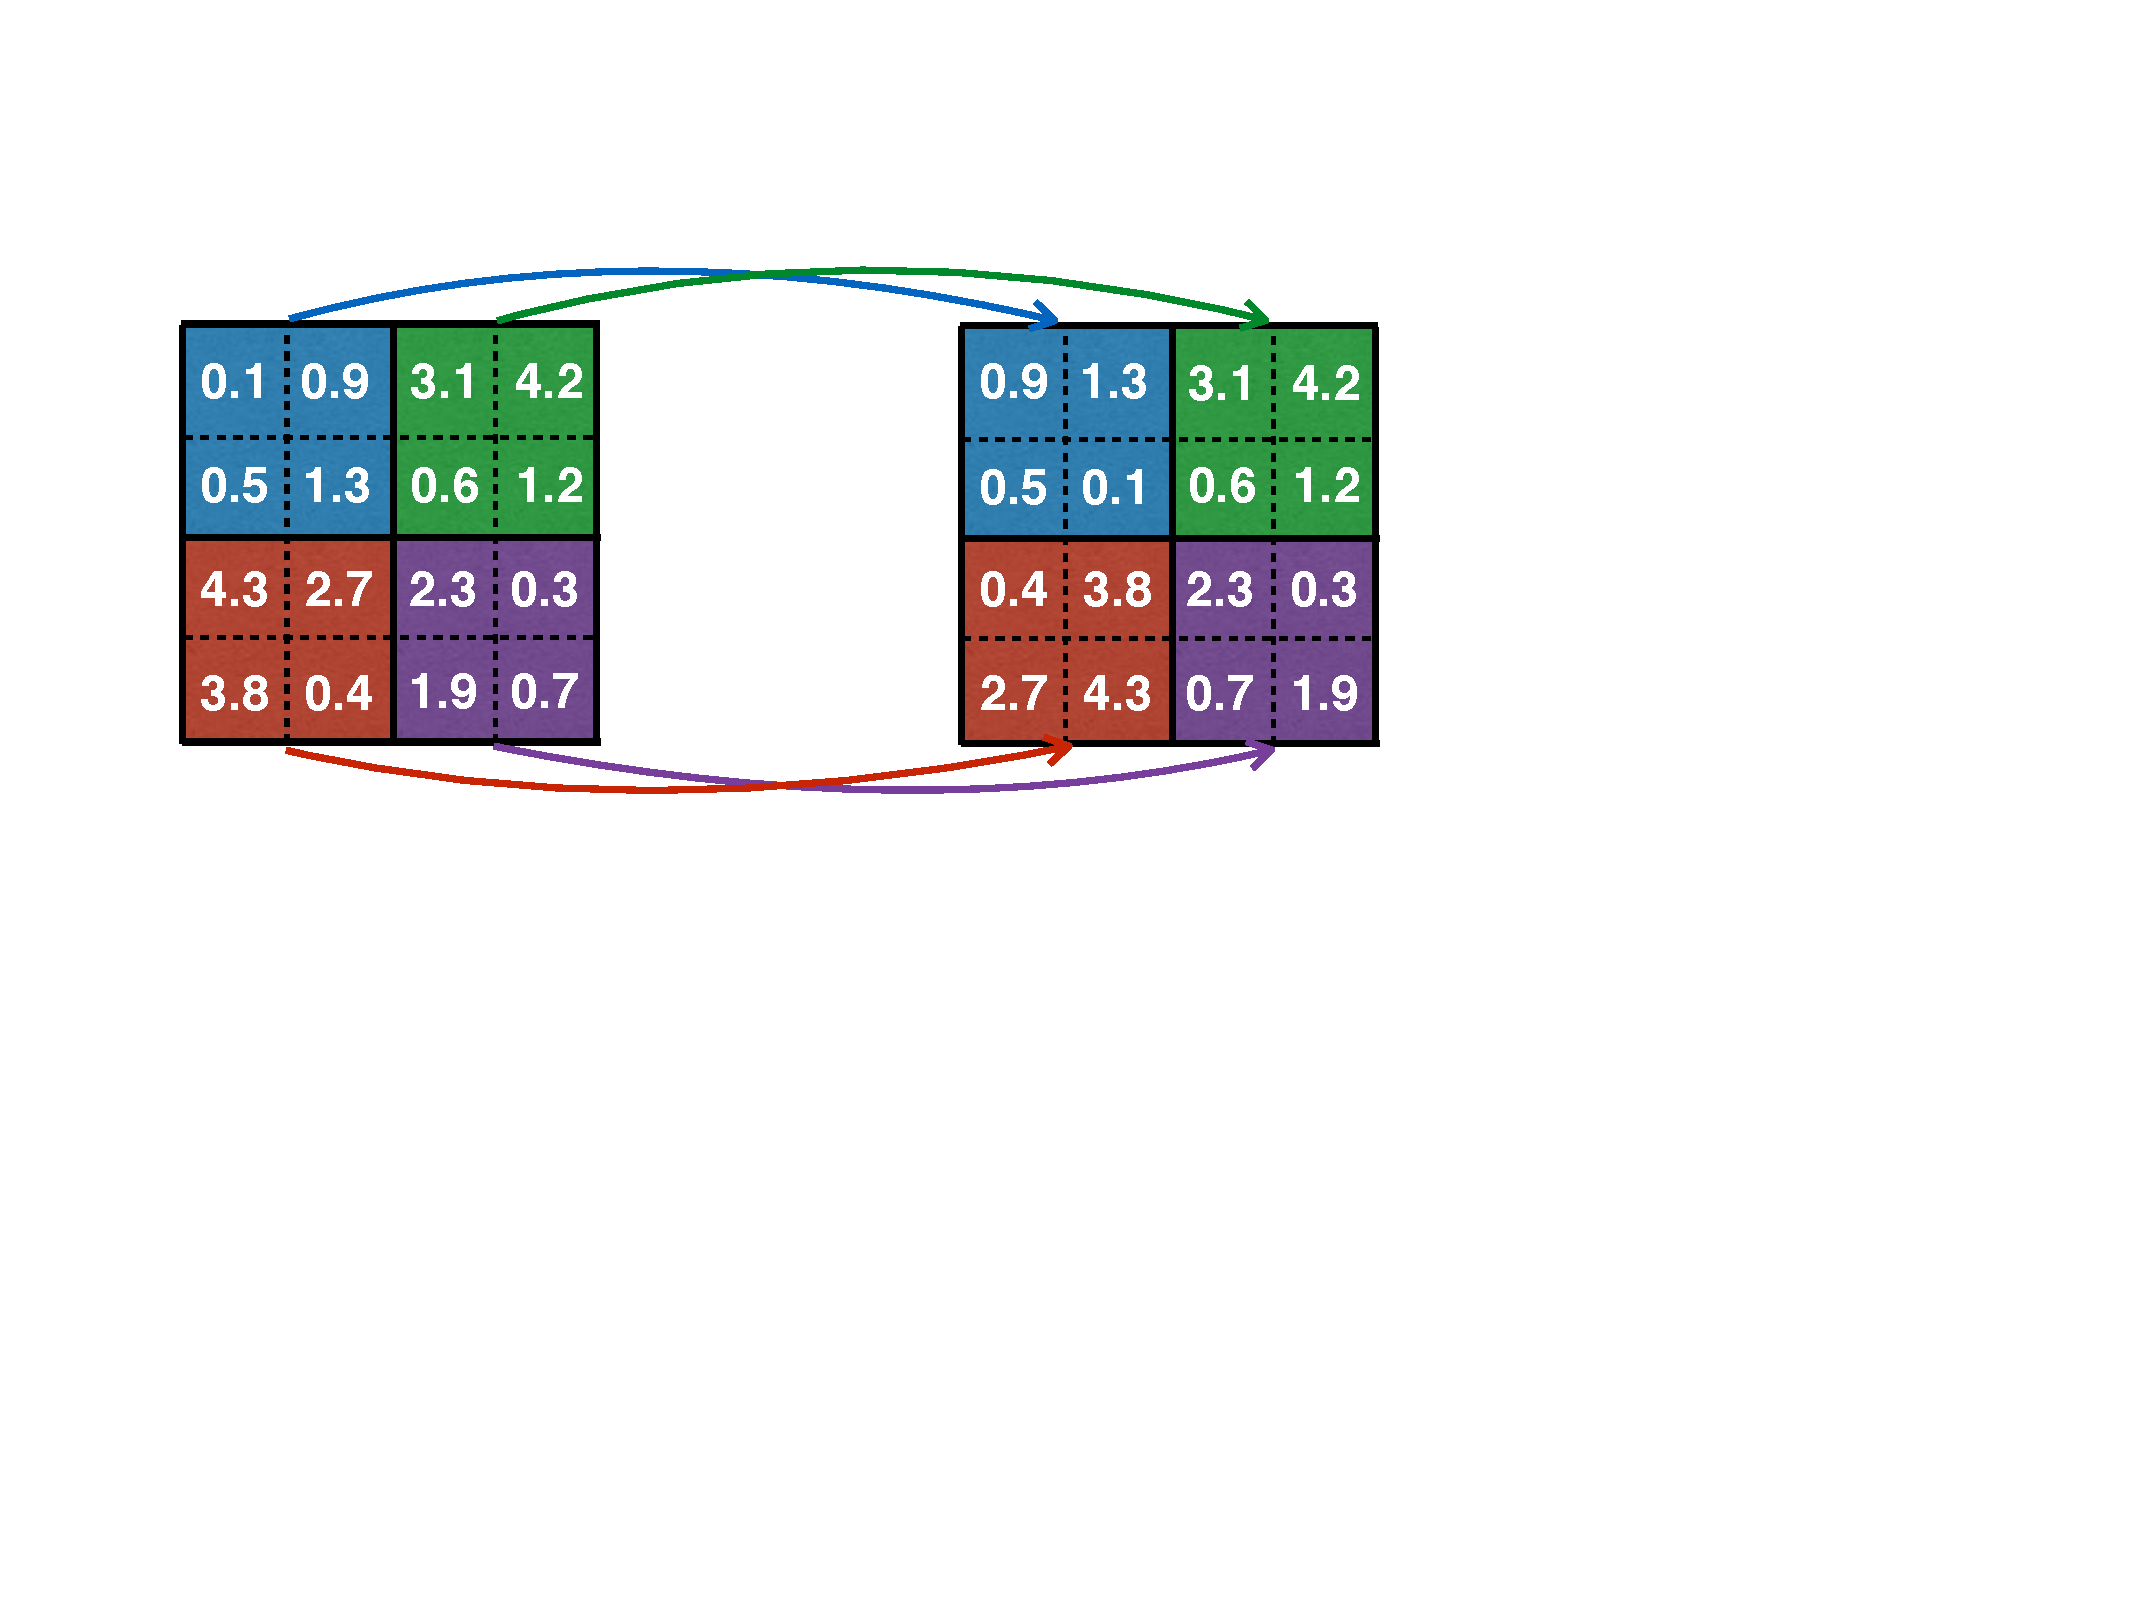
\includegraphics[page=1, width=0.9\textwidth]{./images/PatchShuffle.pdf}
\caption{Simplified illustration of PatchShuffle. A $4 \times 4$ image is split into four $2 \times 2$ patches. Within each patch, pixels are shuffled independently, introducing local variation while preserving the overall image structure~\cite{kang2017patchshuffleregularization}.}
    \label{fig:patchshuffle}
\end{figure}

Figure~\ref{fig:shuffleimages} showcases real-world image samples augmented using PatchShuffle with varying patch sizes. The authors mentioned that PatchShuffle acts as a data augmentation and regularization method. While generated examples maintain the overall global structure of the original input, the internal pixel distributions are altered, making it harder for the model to memorize specific patterns, which is one of the main advantages of the PatchShuffle method. Experimental results demonstrate that PatchShuffle improves classification accuracy and generalization performance across different datasets~\cite{kang2017patchshuffleregularization, hong2024patchmix}.

\begin{figure}[h!]
    \centering
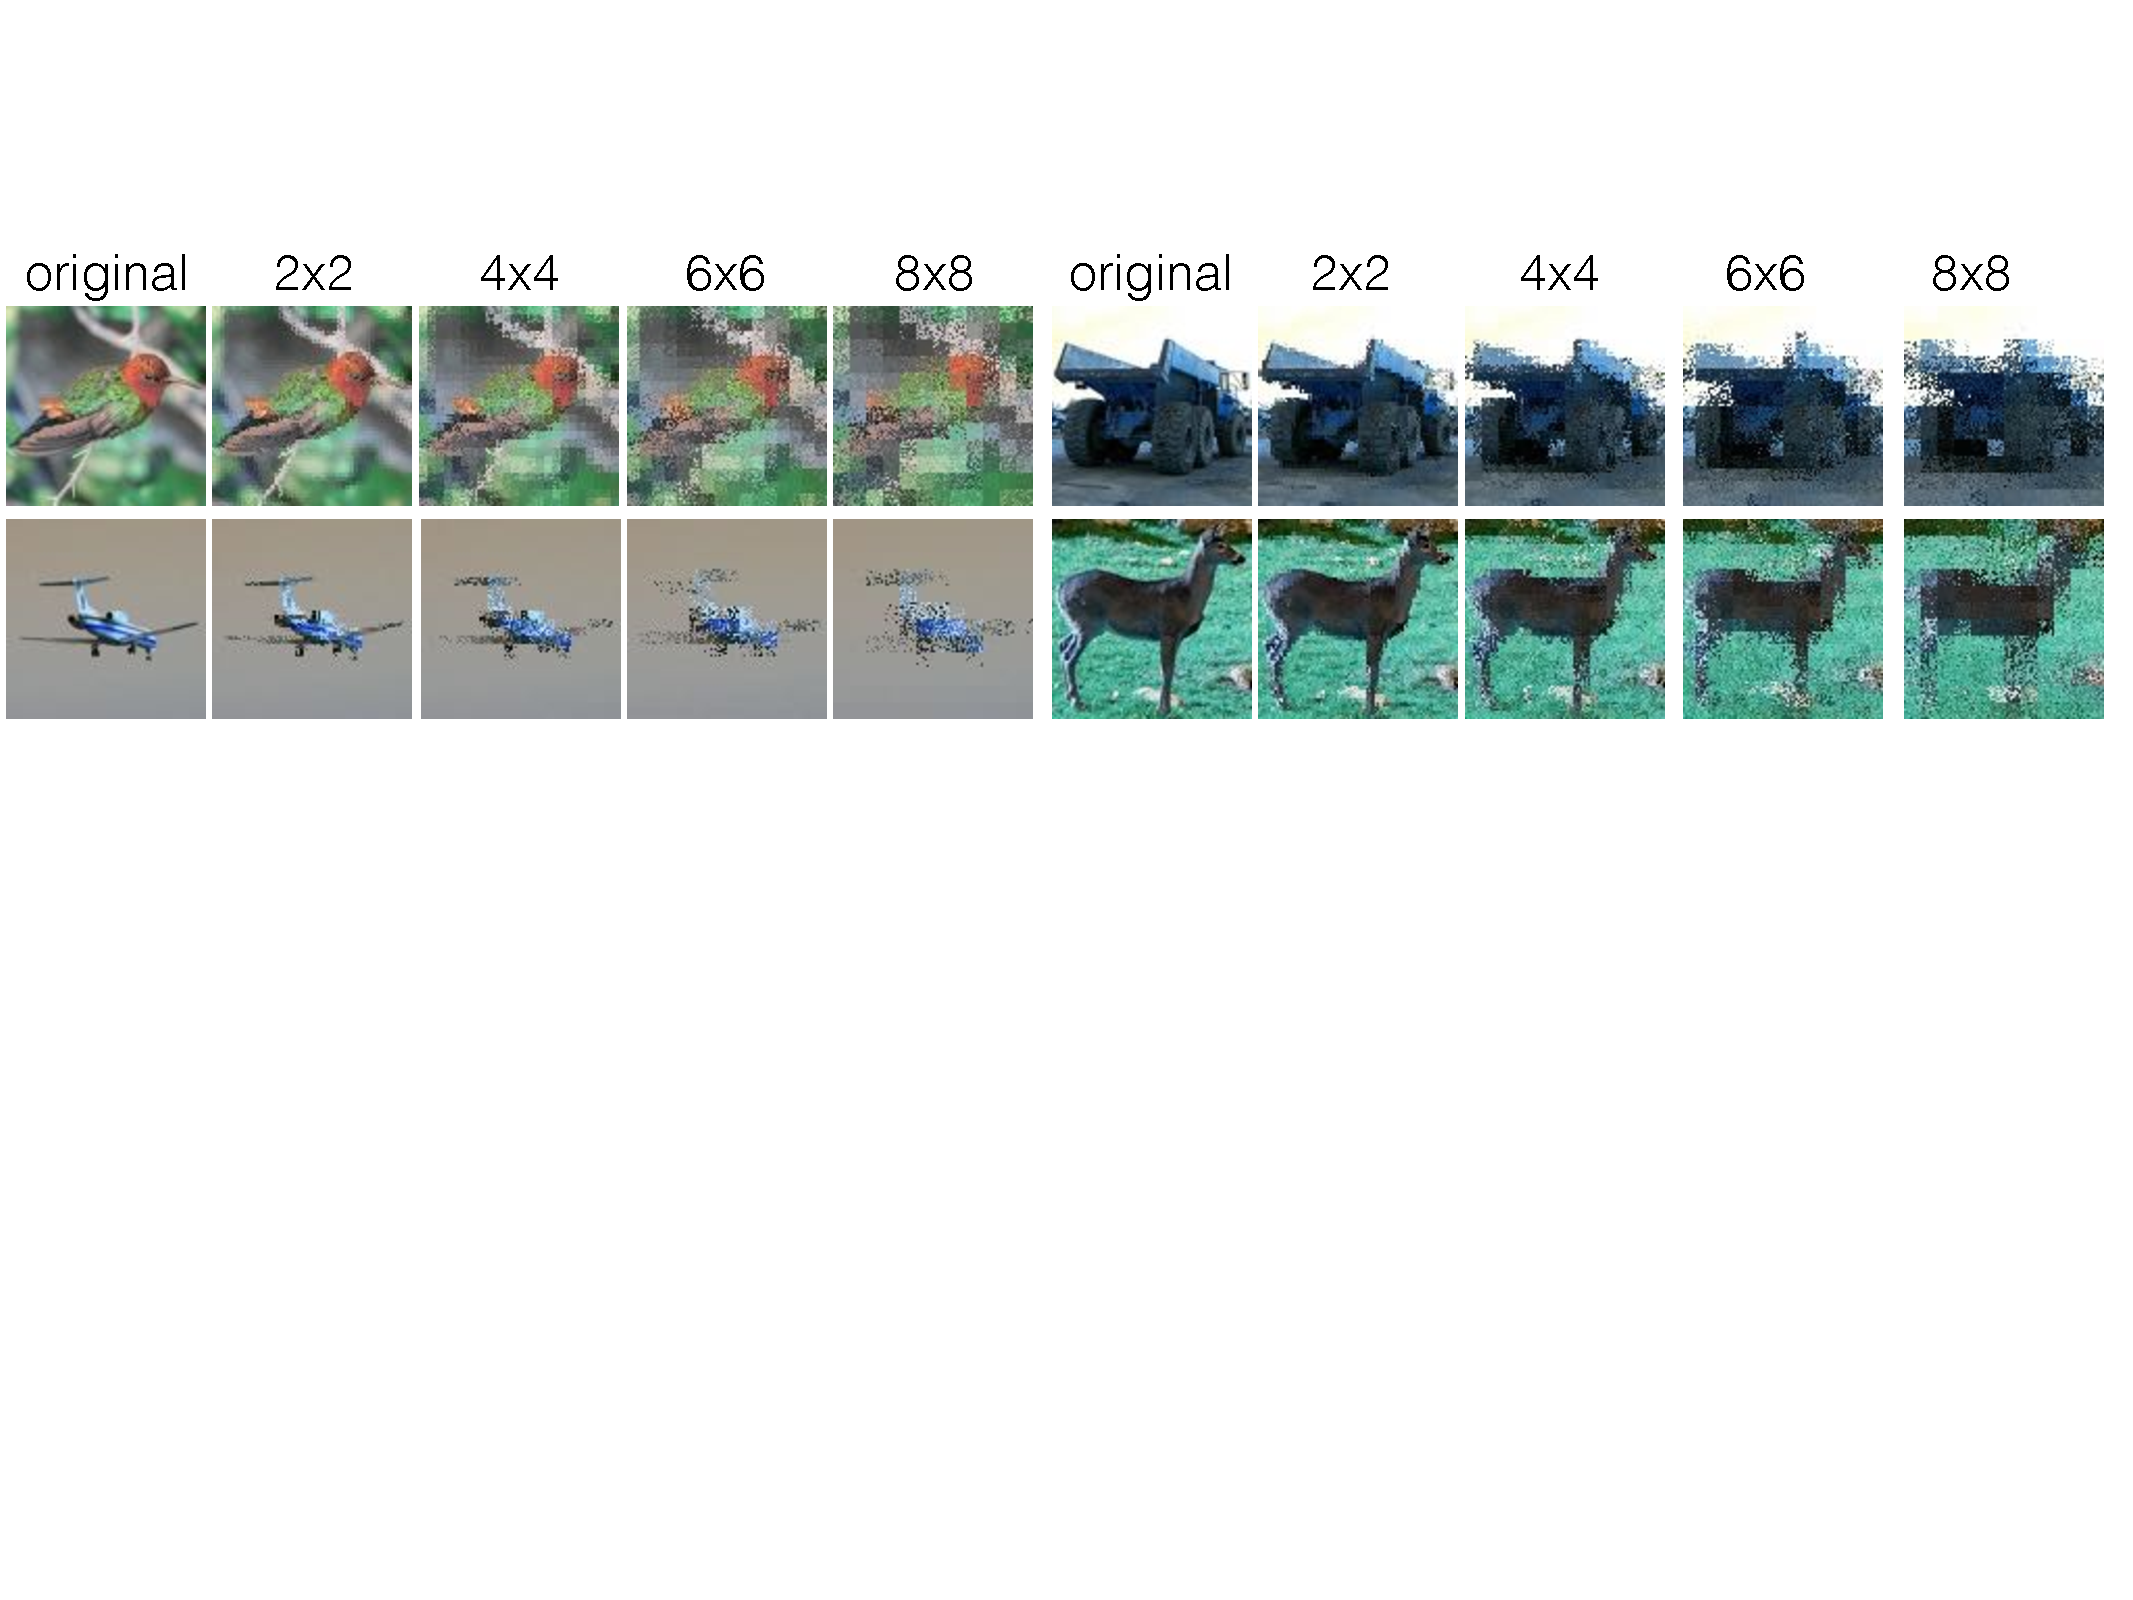
\includegraphics[page=1, width=0.9\textwidth]{./images/ShuffleImages.pdf}
\caption{Real-world image examples augmented with PatchShuffle using different patch sizes. While the global structure is preserved, the internal pixel distribution is altered, promoting regularization and improving generalization by reducing the risk of memorization~\cite{kang2017patchshuffleregularization}.}
    \label{fig:shuffleimages}
\end{figure}



Our proposed method, Temporal Patch Shuffle (TPS), is inspired by patch-based augmentation and regularization techniques developed in the image domain, including PatchShuffle and PatchMix. Nonetheless, applying similar techniques to time series data presents unique challenges. 

Non-overlapping patching and spatial transformations, such as cropping, masking, flipping, etc., are suitable for images as they are structured in a two-dimensional grid. However, they are inappropriate for time series data as they are intrinsically sequential and significantly reliant on temporal order. Transformations such as shuffling or segment reordering can significantly disrupt the temporal dynamics and coherence, potentially worsening performance~\cite{arabi2024wavemaskmixexploringwaveletbasedaugmentations, chen2023fraugfrequencydomainaugmentation}. Our ablation study in Table~\ref{tab:ablation_dlinear} illustrates that using PatchShuffle-style (dividing into non-overlapping patches and shuffling) on time series data results in significantly inferior performance due to the disruption of temporal continuity.

In contrast, our TPS method uses "temporal patches," a concept similarly applied in models like PatchTST~\cite{nie2023timeseriesworth64}, where time series data are partitioned into overlapping segments (patches) with a carefully chosen patch length and stride. These overlapping windows maintain local temporal dependencies and structure to a reasonable degree, even when exposed to transformations such as shuffling. Our ablation study, presented in Figure~\ref{fig:tsne}, utilizes t-distributed Stochastic Neighbor Embedding (t-SNE) visualizations to compare original and augmented samples, supporting our hypothesis that, with appropriately chosen stride and patch length, shuffling patches serves as an effective transformation. It preserves essential signal characteristics while introducing a small amount of functional variability. The results in Table~\ref{tab:dist_metrics} further support these findings.



We propose that this augmentation method, using optimally calibrated parameters, can diminish generalization error, enhance robustness, and reduce variance, similar to the successes of PatchShuffle and PatchMix in image data. Furthermore, we assert that TPS can function as a comprehensive framework for data augmentation within the time series domain. With slight alterations, it can be adapted for various time series tasks, including forecasting and classification.

Sections~\ref{sec: tps_tsf} and \ref{sec:tps_tsc}  describe the specific TPS versions and their applications in time series forecasting and classification, respectively.



\section{TPS for Time Series Forecasting} \label{sec: tps_tsf}



TPS employs the concept of \textit{temporal patches}, where overlapping windows are created using the patch length and stride as hyperparameters within the Temporal Patching block (depicted in green in Figure~\ref{fig:tpstsf}). In the subsequent Variance-Aware Shuffling block (depicted in purple in Figure~\ref{fig:tpstsf}), these patches are sorted in ascending order based on their variance and selectively shuffled according to a predefined \textit{shuffle rate}, $\alpha$. Finally, the augmented sequence is reconstructed by averaging overlapping regions. Before applying the Temporal Patching block, the look-back window and forecast horizon (target) are concatenated like other augmentation methods.

\begin{figure}[h!]
    \centering

\includegraphics[page=1, width=1.0\textwidth, keepaspectratio]{./images/tsf1.drawio.png}
\caption{Illustration of the proposed TPS method for time series forecasting. The input sequence, consisting of a look-back window and a target horizon, is first processed by the \textit{Temporal Patching} block to extract overlapping patches. These patches are then sorted by variance and partially shuffled in the \textit{Variance-Aware Shuffling} block. Finally, the shuffled patches are merged back into a full sequence via the \textit{Reconstruction} block by averaging overlapping regions.}

% {./images/tps_tsf.drawio.png}
    \label{fig:tpstsf}
\end{figure}


Formally, a time series sequence as a combination of look-back window $L$ and forecast horizon $F$ is defined with batch size $B$, sequence length $T$, and number of channels $C$ as:

\begin{equation} \label{eq: concat}
\mathbf{X} = [\mathbf{L}, \mathbf{F}] \in \mathbb{R}^{B \times T \times C}.
\end{equation}


The \textbf{Temporal Patching} block generates patches $\mathbf{P}$ with patch length $p$ and stride $s$ as follows:

\begin{equation} \label{eq: patching}
\mathbf{P} = \text{Unfold}(\mathbf{X}, p, s) \in \mathbb{R}^{B \times N_p \times C \times p},
\end{equation}
where the number of patches $N_p$ is given by:

\begin{equation} 
N_p = \left\lfloor \frac{T - p}{s} + 1 \right\rfloor.
\end{equation}


The \textbf{Unfold} operation extracts patches (sliding windows) from the temporal dimension. The resulting patch tensor is denoted by $\mathbf{P} \in \mathbb{R}^{B \times N_p \times C \times p}$, where $B$ is the batch size, $N_p$ is the number of patches, $C$ is the number of channels, and $p$ is the patch length.

For each sample $b$ in the batch and each patch position $i$, a window of length $p$ is selected starting at temporal position $i \cdot s$ across all channels. This window is then transposed to match the shape $\mathbb{R}^{C \times p}$:
\begin{equation}
\mathbf{P}[b, i] = \left( \mathbf{X}[b, i \cdot s : i \cdot s + p, :] \right)^\top
\end{equation}
This process iterates over all $N_p$ possible patch positions to fill the complete tensor $\mathbf{P}$.


Within the \textbf{Variance-Aware Shuffling} block, importance scores are computed by calculating the variance across the channels and temporal dimension of each patch. For each batch and patch, we first compute the mean across channels and patch temporal elements:
\begin{equation}
\bar{\mathbf{P}}[b, i] = \frac{1}{C \cdot p} \sum_{c=1}^{C} \sum_{j=1}^{p} \mathbf{P}[b, i, c, j]
\end{equation}

Then, the variance is calculated using the correction:
\begin{equation}
\text{Var}(\mathbf{P}[b, i]) = \frac{1}{C \cdot p - 1} \sum_{c=1}^{C} \sum_{j=1}^{p} (\mathbf{P}[b, i, c, j] - \bar{\mathbf{P}}[b, i])^2
\end{equation}

This process generates the importance scores for all patches:
\begin{equation} \label{eq: score}
\text{Score} = \text{Var}(\mathbf{P}) \in \mathbb{R}^{B \times N_p}.
\end{equation}


The number of patches selected for shuffling, $N_s$, is determined by the hyperparameter $\alpha$:

\begin{equation} \label{eq:numberofpatches}
N_s = \left\lfloor \alpha N_p \right\rfloor, \quad \alpha \in (0, 1].
\end{equation}

For each batch, patches are ranked based on their variance scores. Patch indices are sorted, and the indices of the $N_s$ patches with the lowest variance are selected.



\begin{equation} \label{eq: patch_indices}
\mathcal{I} = \{ i_1, i_2, \dots, i_{N_s} \} \subseteq \{1, 2, \dots, N_p\}.
\end{equation}

The selected patches are then randomly shuffled as:

\begin{equation} \label{eq: patchshuffling}
\mathbf{P}_b[\mathcal{I}] = \mathbf{P}_b[\sigma(\mathcal{I})],
\end{equation}
where $\sigma$ denotes a random permutation function applied to the selected indices $\mathcal{I}$.

The \textbf{Reconstruction} block aggregates the shuffled patches by placing each patch back into its original temporal position and averaging overlapping regions. Each patch is positioned according to its stride interval, and when patches overlap due to stride being smaller than patch length, their values are averaged to create a smooth reconstruction. This process generates the final augmented time series: 

\begin{equation}
\mathbf{S} \in \mathbb{R}^{B \times T \times C}.
\end{equation}


$\mathbf{S}$ is partitioned into $\mathbf{S}_L$ and and $\mathbf{S_F}$, where $\mathbf{S_L}$ is concatenated to the original look-back window and $\mathbf{S_F}$ is concatenated to the original target horizon. It follows the same training pipeline as the other augmentations illustrated in Figure~\ref{fig:train_fw}. The pseudocode for TPS is provided in Algorithm~\ref{alg:tps}. 

\begin{algorithm}[H]
\caption{Temporal Patch Shuffle (TPS)}
\label{alg:tps}
\begin{algorithmic}[1]
\REQUIRE Look-back window $\mathbf{L}$ and forecast horizon $\mathbf{F}$, patch length $p$, stride $s$, shuffle rate $\alpha$
\ENSURE Augmented time series $\mathbf{S}$

\STATE $\mathbf{X} \gets \text{Concat}(\mathbf{L}, \mathbf{F})$ \COMMENT{Concatenate input and target sequences}
\STATE $\mathbf{P} \gets \text{Unfold}(\mathbf{X}, p, s)$ \COMMENT{Create overlapping temporal patches}
\STATE $\text{Score} \gets \text{Var}(\mathbf{P})$ \COMMENT{Compute variance-based importance scores}
\STATE $\mathcal{I} \gets \text{Argsort}(\text{Score})[:\alpha \cdot N_p]$ \COMMENT{Select patches with lowest variance}
\STATE $\mathbf{P}[\mathcal{I}] \gets \text{Shuffle}(\mathbf{P}[\mathcal{I}])$ \COMMENT{Shuffle selected patches} \label{alg: shuffle_patches}
\STATE $\mathbf{S} \gets \text{Reconstruct}(\mathbf{P})$ \COMMENT{Reconstruct sequence by averaging overlaps}
\STATE \textbf{return} $\mathbf{S}$
\end{algorithmic}
\end{algorithm}





\section{TPS for Time Series Classification} \label{sec:tps_tsc}


For time series classification, we propose two versions of TPS adapted to the classification setting. Unlike forecasting, where the input consists of both the look-back window and the forecast horizon, classification models only receive the input sequence $\mathbf{X} \in \mathbb{R}^{N \times T \times C}$, where $N$ denotes the number of samples, $T$ the temporal length, and $C$ the number of channels.

The first version of TPS, illustrated in Figure~\ref{fig:tpstsc1}, follows the same procedure as described in Section~\ref{sec: tps_tsf}, with the following modifications:

\begin{itemize}
    \item Instead of concatenating the input and forecast horizon, only the raw input $\mathbf{X}$ without labels is used.
    \item The shuffling process is applied at the \textit{sample level} rather than the batch level; that is, TPS is applied independently to each sample. The batch dimension $B$ is replaced by the sample dimension $N$ in our formulation.
\end{itemize}

For classification, we apply edge-value padding to ensure full patch coverage. This differs from the forecasting setting, where padding is omitted. The pseudocode for this version follows the structure of Algorithm~\ref{alg:tps}, incorporating the modifications listed above.


\begin{figure}[h!]
\centering

\includegraphics[page=1, width=1.0\textwidth, keepaspectratio]{./images/tsctps.png}
\caption{Illustration of the first version of the proposed TPS method for time series classification. This version adapts the forecasting design by applying Temporal Patching and Variance-Aware Shuffling at the sample level, using only the input data without class labels.} 
    \label{fig:tpstsc1}
\end{figure}


The second version, \textbf{Temporal Index Patch Shuffle (TIPS)}, extends TPS by introducing patch-level index shuffling \textit{across samples of the same class}. Rather than reusing patches from the same sample, this version replaces selected patches with patches from other random samples sharing the same class label.

Formally, given labels $Y \in \mathbb{R}^{N}$ or one-hot encoded labels $\mathbf{Y} \in \mathbb{R}^{N \times K}$, for each sample $i$ with label $y_i$, we define the set of other samples with the same label as:

\begin{equation}
\mathcal{N}_i = \left\{ j \in \{1, \dots, N\} \,\middle|\, y_j = y_i,\ j \ne i \right\}.
\end{equation}

For each selected patch index $P_k$ in sample $i$, we randomly select a sample $j \in \mathcal{N}_i$, extract the patch from the same temporal location, and use it to replace the corresponding patch in sample $i$. This replacement is repeated $N_s$ times for each patch that needs to be shuffled. The procedure introduces semantic diversity while preserving class consistency. To maintain dimensional consistency, edge-value padding is applied when necessary. An illustration of this process is provided in Figure~\ref{fig:tpstsc2}.



\begin{figure}[h!]
    \centering
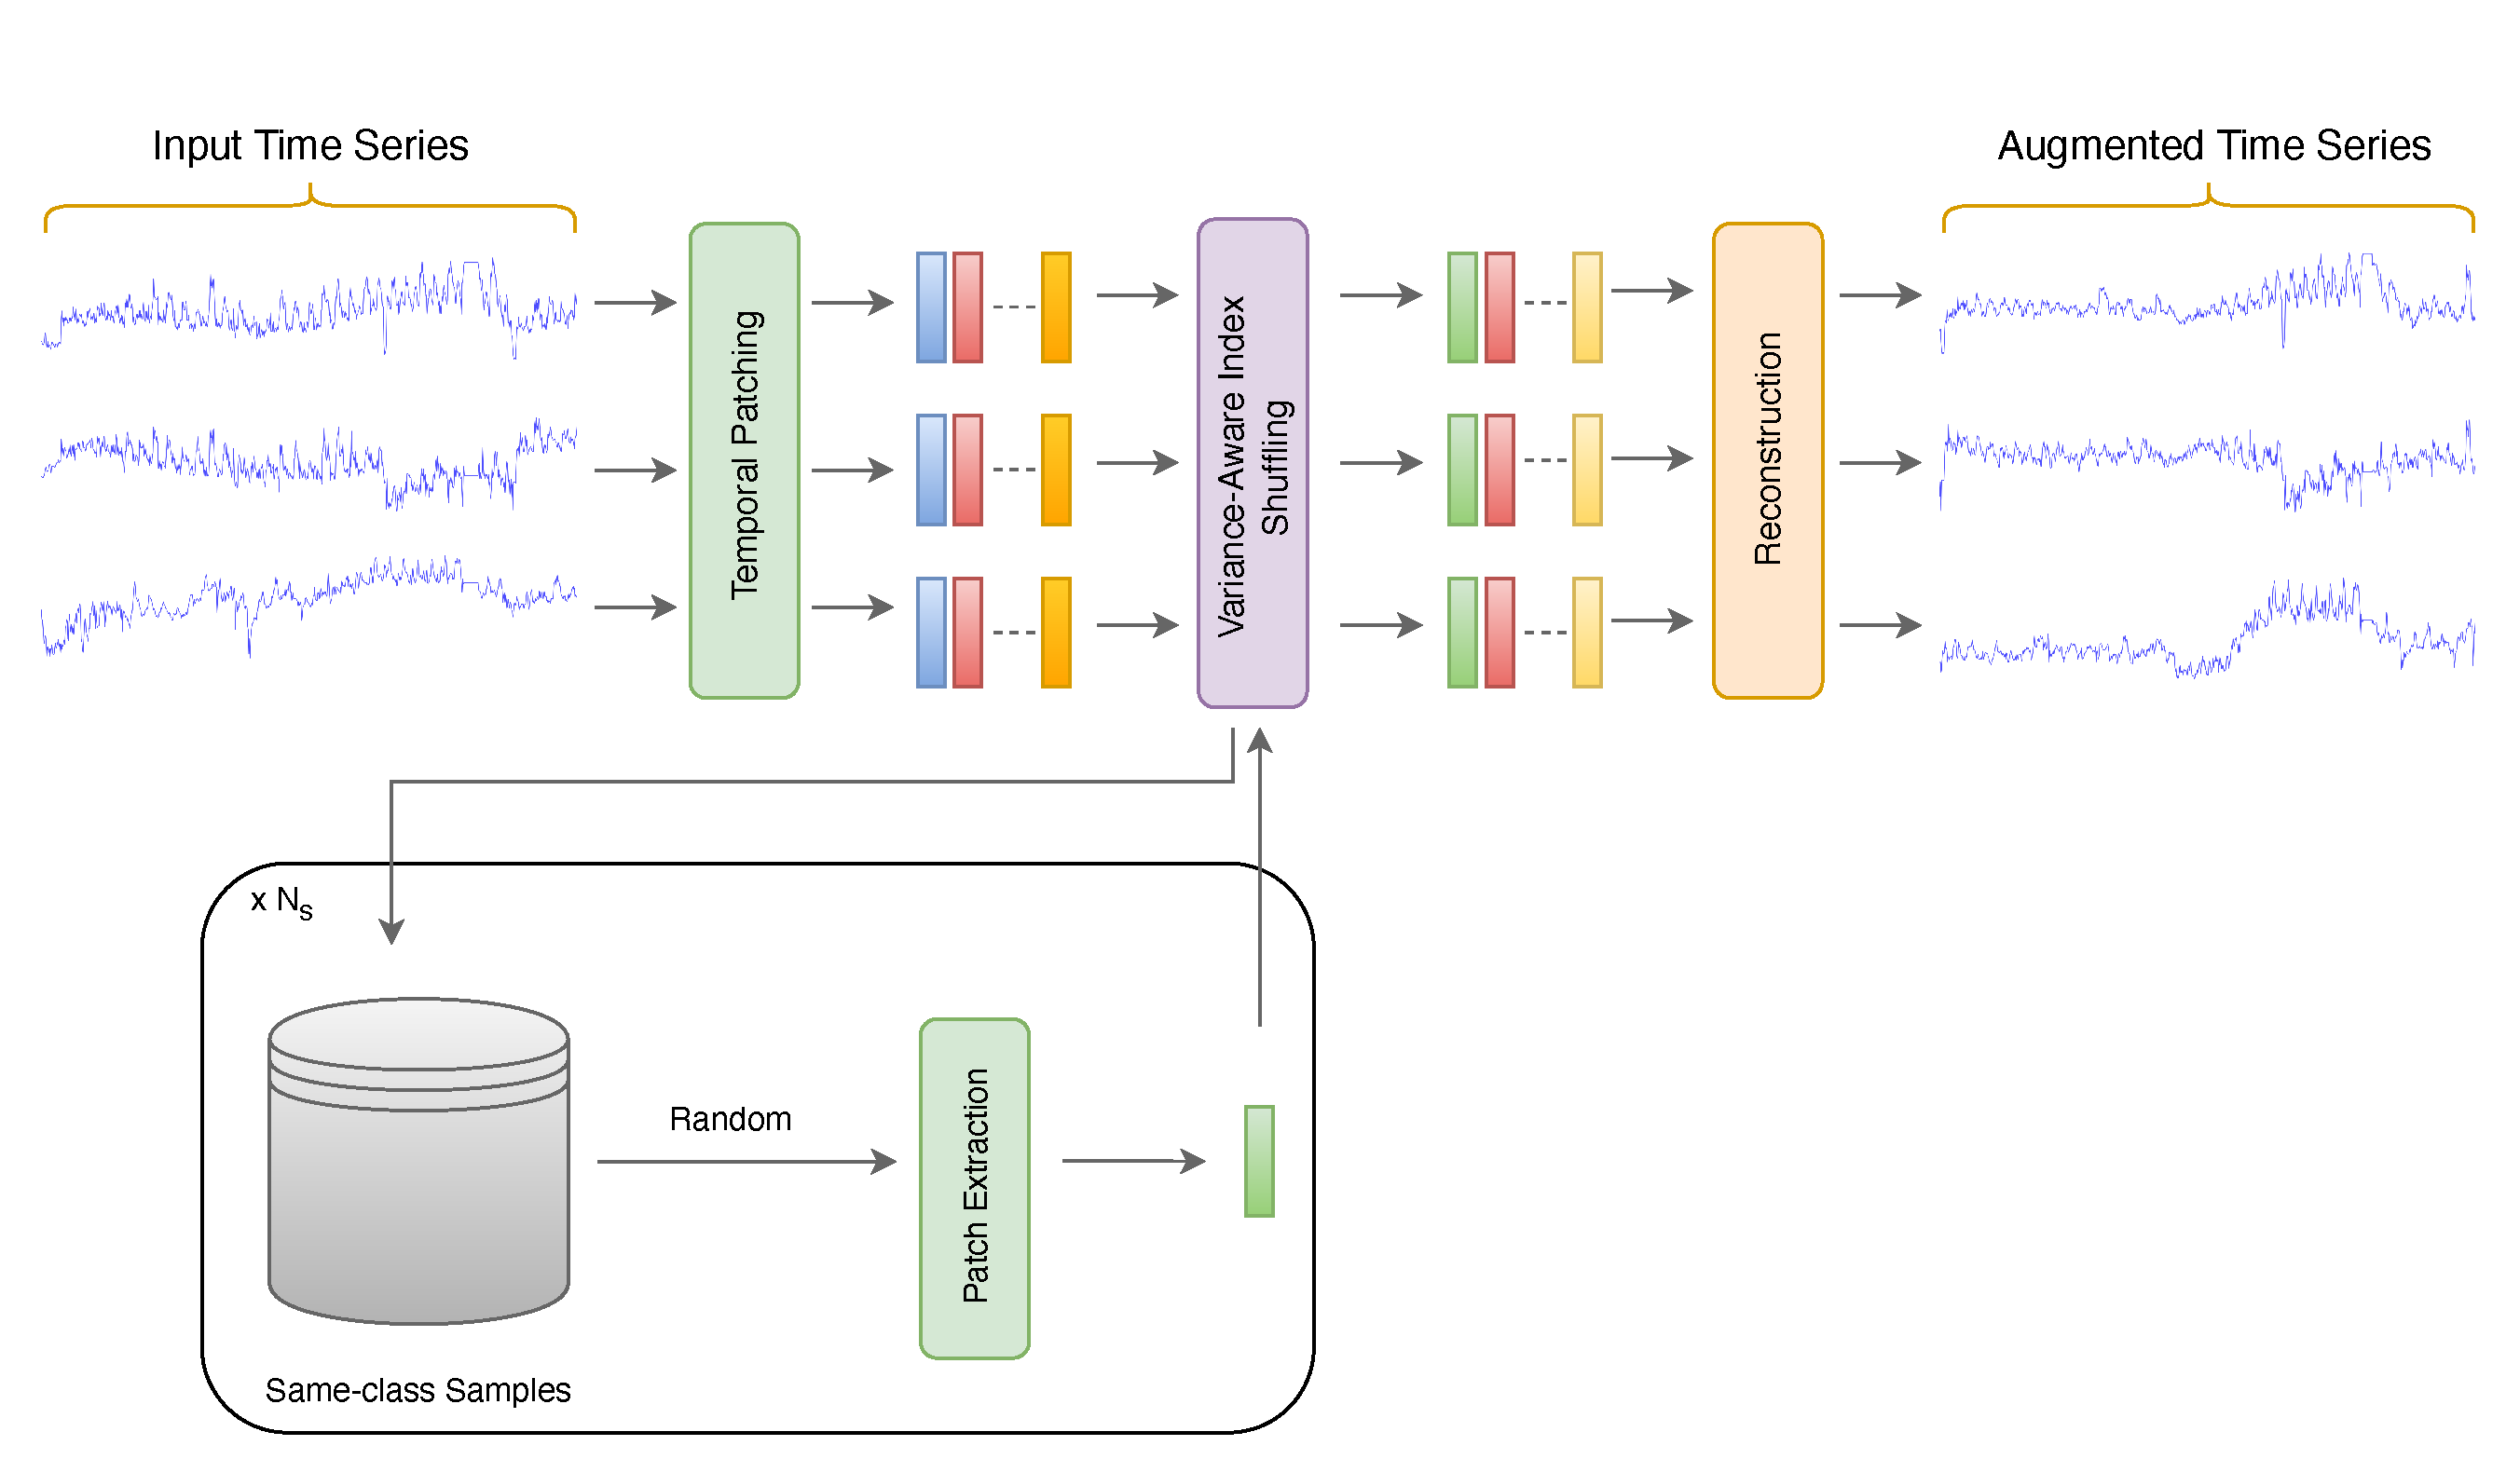
\includegraphics[page=1, width=1.0\textwidth, keepaspectratio]{./images/tps_tsc.drawio2.drawio.pdf}
\caption{Illustration of the second version of the proposed method, \textbf{Temporal Index Patch Shuffle (TIPS)}, for time series classification. Unlike the first version of TPS, TIPS introduces patch-level shuffling \emph{across samples with the same class label}. For each selected patch within a sample, TIPS replaces it with a patch from the same temporal location of a randomly selected sample belonging to the same class}

    \label{fig:tpstsc2}
\end{figure}

The pseudocode for TIPS is presented in Algorithm~\ref{alg:tps_class}. The key difference from the original version lies in Lines~\ref{alg: same-class}–\ref{alg: cross_patch}, which implement an additional step: extracting patches from a randomly selected sample belonging to the same class as the current instance (illustrated in Figure~\ref{fig:tpstsc2}). In contrast, the original version (Algorithm~\ref{alg:tps}) uses a simpler shuffling operation, represented by Line~\ref{alg: shuffle_patches}, without involving any cross-sample interactions. It is also important to note that, in practice, all operations for the classification setting are applied in a per-sample sequential manner. These two versions for classification tasks follow the training pipeline in Figure~\ref{fig:tsc_fw}, the same as other augmentation methods.



\begin{algorithm}[H]
\caption{Temporal Index Patch Shuffle (TIPS)}
\label{alg:tps_class}
\begin{algorithmic}[1]
\REQUIRE Input sequence $\mathbf{X} \in \mathbb{R}^{N \times T \times C}$, labels $Y \in \mathbb{R}^N$, patch length $p$, stride $s$, shuffle rate $\alpha$
\ENSURE Augmented time series $\mathbf{S} \in \mathbb{R}^{N \times T \times C}$

\STATE $\mathbf{P} \gets \text{Unfold}(\mathbf{X}, p, s)$ \COMMENT{Create overlapping patches for each sample}
\STATE $\text{Score} \gets \text{Var}(\mathbf{P})$ \COMMENT{Compute variance-based scores per sample}
\STATE $N_s \gets \lfloor \alpha \cdot N_p \rfloor$ \COMMENT{Determine number of patches to shuffle per sample}

\FOR{each sample $i \in \{1, \dots, N\}$}
    \STATE $\mathcal{I}_i \gets \text{Argsort}(\text{Score}_i)[:N_s]$ \COMMENT{Select low-variance patch indices}
    \STATE $\mathcal{N}_i \gets \{ j \in \{1, \dots, N\} \mid y_j = y_i,\ j \ne i \}$ \COMMENT{Find same-class neighbors} \label{alg: same-class}
    \FOR{each index $k \in \mathcal{I}_i$}
        \STATE $j \gets \text{RandomSample}(\mathcal{N}_i)$ \COMMENT{Randomly select same-class sample}
        \STATE $\mathbf{P}_i[k] \gets \mathbf{P}_j[k]$ \COMMENT{Replace patch from same temporal location} \label{alg: cross_patch}
    \ENDFOR
\ENDFOR

\STATE $\mathbf{S} \gets \text{Reconstruct}(\mathbf{P})$ \COMMENT{Reconstruct sequence by averaging overlaps}
\STATE \textbf{return} $\mathbf{S}$
\end{algorithmic}
\end{algorithm}



TPS can be applied to other time series domains with minimal adaptation to task-specific properties. One example is self-supervised models, which typically rely on other augmentations to improve accuracy or reduce errors. We will discuss this in more detail in Section~\ref{sec:future}.


\section{Methodological Rationale \& Design Objectives} \label{sec:method_design}

The design of our proposed method, \textbf{TPS (Temporal Patch Shuffle)}, is grounded in three key objectives: (1) preserving temporal coherence, (2) introducing controlled variability, and (3) maintaining data-label consistency. Unlike image data, time series are highly sensitive to temporal ordering; thus, transformations must avoid disrupting sequential structure.

TPS introduces three tunable parameters—patch length, stride, and shuffle rate—that allow users to flexibly generate either samples closely resembling the original data or augmented sequences with meaningful variability. This facilitates both improved generalization and reduced overfitting. Our ablation studies in Chapter~\ref{chapter:experiments} (see Figure~\ref{fig:tsne} and Table~\ref{tab:dist_metrics}) empirically support these claims.

One component of TPS is \textbf{low-variance patch sorting}, which prioritizes the shuffling of patches with low temporal variability, as they are less critical to the sequence’s temporal structure. In contrast, random selection may disrupt meaningful patterns, particularly in certain datasets and prediction lengths where the shuffle rate is not 1.0. Moreover, the use of \textbf{overlapping patches}—as also utilized in models like PatchTST~\cite{nie2023timeseriesworth64}—helps preserve local dependencies better than non-overlapping alternatives. The final step of \textbf{reconstruction} acts as an implicit smoothing or denoising process, where overlapping regions are averaged to restore the sequence. All of these aspects will be discussed in detail in Section~\ref{sec:ablation}.

In the classification context, we introduce \textbf{TIPS (Temporal Index Patch Shuffle)} as an extension of TPS. This version incorporates \textbf{cross-sample patch exchange} by replacing selected patches with those from other samples within the same class. This is feasible for classification, as samples from the same class can share structural information; however, it is inapplicable to forecasting due to the nature of prediction targets. As demonstrated in Chapter~\ref{chapter:experiments}, TIPS achieves superior performance in both univariate and multivariate classification, outperforming even the original TPS. This highlights the flexibility of our framework: with minimal modifications, it can be adapted for different tasks and objectives.

Both TPS and TIPS are designed to be lightweight and scalable. The primary computational cost stems from patch extraction and shuffling. Since these operations are non-parametric, they can be efficiently integrated into the training pipeline as \textbf{on-the-fly augmentations}, adding minimal overhead in training time or memory usage. To quantify this, we present runtime comparisons for augmentation in Tables~\ref{tab:augmentation_comparison} and \ref{tab:aug_times_tsc}, which focus on forecasting and classification, respectively.

One limitation of TPS and TIPS is the requirement to tune three hyperparameters to match the characteristics of a given dataset. However, according to Figure~\ref{fig:ablation_lightts} in the ablation study, a higher shuffle ratio, moderate patch length, and lower strides generally lead to lower generalization error, which can help us reduce our hyperparameter search cost. In Section~\ref{sec:future}, we explore adaptive patch sizing and other potential enhancements to TPS.

Overall, we have thoroughly evaluated both TPS and TIPS across various models and scenarios in the next chapter. Our ablation studies validate the effectiveness of the proposed design principles. 





